\chapter{Integrated Circuitry Design}
This chapter presents the design of the read-out circuit and the post-simulation results.


\section{Fronted Circuit Design}
The review of the source follower in section.\ref{section:SF} suggests the constant current method for the circuit of DC-sweep mode.
The data analysis from chapter 3 supports it by the linear relation between $I_D$ and $g_m$.
However, section.\ref{sec:AC} shows that source follower is not suitable for transient measurement.
It alternatively recommends the circuit in Fig.\ref{fig:lockin} which measures the transient current signal and converts it into a voltage output.

The fronted circuit combined these two methods into one circuit structure with two modes available: DC-sweep mode and Transient Measurement mode.

\subsection{The Circuit of DC-sweep mode}
\begin{figure}[!htbp]
    \centering
    \includegraphics[width=0.5\textwidth] {images/chapter5/DCMode.png}
    \caption{The fronted circuit operated in DC-sweep mode.}
    \label{fig:DCmode}
\end{figure}
Fig.\ref{fig:DCmode} is the fronted circuit operated in DC-sweep mode.
The switch turns the circuit into DC-sweep mode by connecting the output of OP with the gate of nanowire.

As in the source follower, our circuit contains a biasing current source (Ibias) for controlling the $I_D$.
The difference is that the Ibias inputs the current into drain instead of source.
In addition, we employs the transimpedance amplifier (TIA) from section.\ref{sec:AC} (\cite{Jlockin}).
Its output is connected to an OP amplifier to form a negative feedback loop.
When $I_D$ is less than Ibias, the output voltage of TIA falls and the gate voltage $V_G$ rises to increase $I_D$.
On the contrary, output voltage of TIA rises and the gate voltage ($V_G$) drops if Ibias is smaller than $I_D$.
Finally, the feedback mechanism forces $I_D$ to be the same as Ibias by adjusting $V_G$ automatically.


\subsection{The Circuit and Usage of Transient Measurement mode} \label{sec:TrM}

\begin{figure}[!htbp]
    \centering
    \begin{minipage}[t]{0.45\textwidth}
        \includegraphics[width=1\textwidth] {images/chapter5/ACMode.png}
        \raggedleft
        (a)
    \end{minipage}
    \hfill
    \begin{minipage}[t]{0.45\textwidth}
        \includegraphics[width=1\textwidth] {images/chapter5/ACMode_sine.png}
        \raggedleft
        (b)
    \end{minipage}
    \caption{Two usage (\textbf{(a)}, \textbf{(b)}) of the fronted circuit operated in Transient Measurement mode.}
    \label{fig:ACmode}
\end{figure}

In Fig.\ref{fig:ACmode}(a), the switch turns to a simple voltage source (Vg) that provides a constant gate voltage.
The feedback OP is nonfunctional in this mode.
When performing measurement, we directly find how the output voltage ($V_{out}$) changes with the biomolecule concentration.
This output voltage will be sent into a second stage circuit for further amplification.

\paragraph*{Another Usage of Transient Measurement mode}
There is another method to perform measurement with Transient Measurement mode, which resembles the measurement in \cite{Jlockin}.
This method measures the $g_m$ of the nanowire.
As shown in Fig.\ref{fig:ACmode}(b), a sinusoidal signal with an amplitude of $v_s$ is sent to the source of the nanowire.
The output response ($V_{out}$) is a sinusoidal signal at the same frequency with an amplitude equaling to $v_sg_m \times R_{TIA}$.
The values of Ibias and Vg can be arbitrary.
But one need to be aware that their values should not cause the output of TIA or the second-stage circuit to saturate.

\subsection{The Variability-resisting method}
As mentioned in chapter 1, we combine DC-sweep mode and Transient Measurement mode to implement the variability-resisting measurement method.

\paragraph*{Method Procedure}
Assuming there are two nanowire devices and the device variability problem exists between them.
Initially, we use these element to perform the $I_D$-$V_G$ sweep in DC-sweep mode.
We use the $I_D$-$V_G$ curve to find the $g_m$ of each device. ($g_m = \frac{\partial I_D}{\partial V_G}$)
When we turns to Transient Measurement mode, we bias these two devices under the same $g_m$ by setting Ibias and Vg correspondingly.
After the buffer solutions, the same voltage difference at the output ($V_{out}$) should be detected because the two devices have the same $g_m$.
Before a new solution is added, we return to DC-sweep mode again.
This is for finding the new biasing $V_G$ to reset their $I_D$ to be the same as Ibias.
This implies that every time when we enter Transient Measurement mode, the devices always have the same $I_D$ and $g_m$ as those in the beginning of experiments.


\subsection{Design Description}
In this section, we first talk about TIA block and focus on how we improve the detecting limits of this block.
It is followed by the design of the TIA circuit.
Then we analyze the feedback mechanism of DC-sweep mode and the input impedance of the circuit.
After that, we discuss the stability issue.
Finally, we show the design of the feedback OP block.

\subsubsection{Strategies for lowering current detecting limits} \label{sec:Ibias}
The TIA subcircuit in section.\ref{sec:ch2CC} is shown as Fig.\ref{fig:TIA_old}(a), we mentioned that the detecting range of $R_{NW}$ is limited by $I_{NW}$ provided by TIA.
We now discuss the causes of the upper and lower limits, and show the strategies we use to improve them.

\begin{figure}[!htb]
    \centering
    \begin{minipage}[t]{0.45\textwidth}
        \includegraphics[width=1.1\textwidth] {images/chapter5/TIA_olda.png}
        (a)
    \end{minipage}
    \hfill
    \begin{minipage}[t]{0.45\textwidth}
        \includegraphics[width=1\textwidth] {images/chapter5/TIA_old.png}
        (b)
    \end{minipage}
    \caption{\textbf{(a)} The transimpedance block (TIA) of the read-out circuit from \cite{Jlockin}. The circuit input a voltage signal into resistive nanowire element $R_{NW}$.
            To compare it with our circuit (Fig.\ref{fig:TIA}), we transform the voltage input into an equivalent current input in \textbf{(b)}. The $I_{NW} = (V_{Ref} - V_{in})/R_{NW}$ and $\Delta i = \Delta vi /R_{NW}$}
    \label{fig:TIA_old}
\end{figure}

\paragraph*{Lower Limit:}
In Fig.\ref{fig:TIA_old}(b), the TIA output voltage is:
\begin{equation}
    V_{TIA} = V_{Ref} + I_{NW}R_{TIA} + \Delta iR_{TIA}
    \label{eq:TIA_old}
\end{equation}
Two reasons relate to a large offset current $I_{NW}$.
One is that the output current provided by TIA is restricted by design.
The other is that the restriction of the current flowing through the resistor $R_{TIA}$:
\begin{align}
    \frac{V_{Ref} - VSS}{R_{TIA}} < I_{NW} < \frac{VDD - V_{Ref}}{R_{TIA}}
\end{align}
Both reasons lead to the output saturation of TIA.

A naive way to handle the first one is to increase the maximal output current that TIA can provide.
The disadvantage of this method is the increase in power consumption and chip area.
As for the second one, using smaller $R_{TIA}$ can release the restriction on $I_{NW}$.
Unfortunately, this is not preferred because it reduces the current-to-voltage gain of TIA.

Our strategy for decreasing the lower limit is to utilize the biasing current source (Ibias) of nanowire.
As shown in Fig.\ref{fig:TIA}, Eq.(\ref{eq:TIA_old}) is transformed into:
\begin{equation}
    V_{TIA} = V_{Ref} + (I_{NW} - I_{bias}) R_{TIA} + \Delta iR_{TIA}
    \label{eq:TIA}
\end{equation}
Now we can diminish the large $I_{NW}$ by Ibias.

In conclusion, the large offset current causes the saturation of the output of TIA.
We use the biasing current source to diminish that offset current, so as to increase the detection range.

\begin{figure}[!htbp]
    \centering
        \includegraphics[width=0.4\textwidth] {images/chapter5/TIA.png}
    \caption{}
    \label{fig:TIA}
\end{figure}
\paragraph*{Upper Limit:}
The upper limit depends on the output resolution.
When the input current signal $\Delta I$ in Fig.\ref{fig:TIA} is too small, the output response may be defeated by the noise.
This may be solved by increasing the SNR through a larger $R_{TIA}$.
{However, the chip area constrains the size of resistors.
In our circuit design, it is hard to make a wide linear range resistor with resistance value out of $100k\Omega$.
Furthermore, even if the resistor can be greater, one needs to concern for the noise brought by the large resistance.

Our strategy is to reduce the noise of TIA by designing its input MOSFETs with a large area.
We also amplify the output signal through the second-stage circuit.

\subsubsection{TIA (Transimpedance Amplifier) Design}

\begin{figure}[!htb]
    \centering
    \begin{minipage}[t]{0.4\textwidth}
        \includegraphics[width=1\textwidth] {images/chapter5/TIA_block.png}
        \raggedleft
        (a)
    \end{minipage}
    \hfill
    \begin{minipage}[t]{0.5\textwidth}
        \includegraphics[width=1\textwidth] {images/chapter5/TIA_sch.png}
        \raggedleft
        (b)
    \end{minipage}
    \caption{\textbf{(a)} The transimpedance block and the \textbf{(b)} schematic}
    \label{fig:TIA_sch}
\end{figure}

\begin{figure}[h!tb]
    \centering
        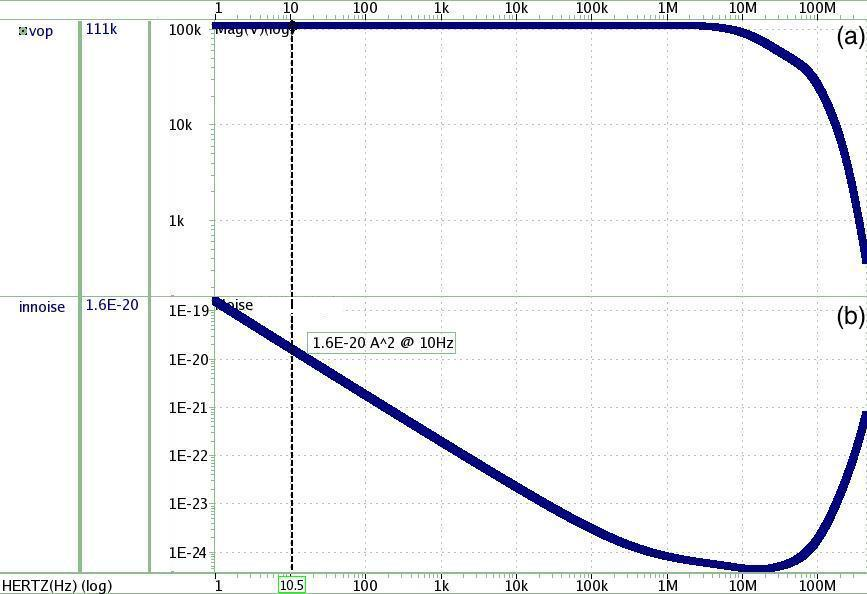
\includegraphics[width=0.8\textwidth] {images/chapter5/postSim/TIA_ac.jpg}
    \caption{The ac simulation results of TIA. The x-axis is the input signal frequency. \textbf{(a)} is the $V_{out}$ and \textbf{(b)} is the input-referred noise (A\^2).}
    \label{fig:TIA_postSim_ac}
\end{figure}

\emphy{Fig.\ref{fig:TIA_sch} shows the Transimpedance Amplifier circuit.
We implement the operational amplifier in TIA with the two-stage, differential-pair structure.
This simple structure has merits such as large output current and wide output voltage range.}



\begin{figure}[tb]
    \centering
        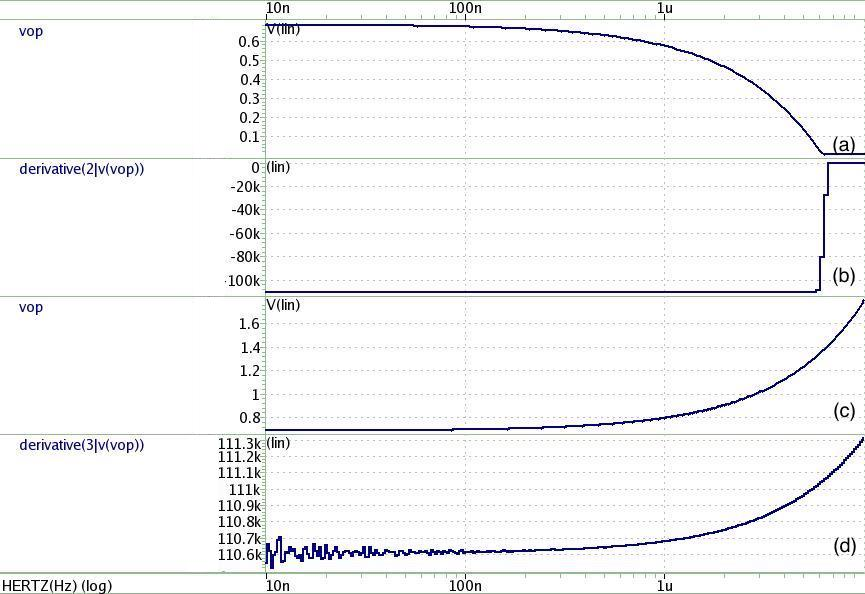
\includegraphics[width=0.9\textwidth] {images/chapter5/postSim/TIA_dc.jpg}
    \caption{The dc simulation results of TIA. The x-axis represents positive/negative input current (log scale). \textbf{(a)} is the $V_{out}$ responding to the positive input current while \textbf{(c)} is to the negative input current.
                    \textbf{(b)} and \textbf{(d)} are the derivative of $V_{out}$ of input current ($\frac{\partial V_{out}}{\partial {I_{in}}}$) from \textbf{(a)} and \textbf{(c)} respectively.}
    \label{fig:TIA_postSim_dc}
\end{figure}





\emphy{Fig.\ref{fig:TIA_postSim_ac} and Fig.\ref{fig:TIA_postSim_dc} are the ac and dc post-simulation of TIA.
Fig.\ref{fig:TIA_postSim_ac}(a) indicates that the bandwidth is $7M Hz$.
Fig.\ref{fig:TIA_postSim_ac}(b) is the input referred noise.
Fig.\ref{fig:TIA_postSim_dc} shows that TIA has a constant transimpedance of $100k \Omega$ when the input current range is $6\mu A \sim -10\mu A$.
In Table.\ref{tb:TIAsim}, these three parameters are compared with the specification given by Table.\ref{tb:ACSpec}.
Other results such as biasing current, spec. of OP ... etc. are also provided in it.}


\begin{table}[!htb]
    {\fontfamily{}\fontsize{10}{14}\selectfont
    \centering
    \begin{tabular}{l|c|c}
        VDD & \multicolumn{2}{c}{$3.3V$} \\
        \hline
        Biasing Current & \multicolumn{2}{c}{$35\mu A$} \\
        \hline
        Transimpedance & \multicolumn{2}{c}{$100k (\frac{V}{I})$} \\
        \hline
        \hline
        \multicolumn{3}{c}{Closed loop} \\
        \hline
        & Post-simulation & Spec. from Table.\ref{tb:ACSpec} \\
        \hline
        Input Current range & from $6\mu A$ to $-10\mu A$ & $\pm$ $20n A$ - $2.8\mu A$\\
        \hline
        Output Voltage range &$0.1V$ - $2.8V$ & - \\
        \hline
        Bandwidth &7M Hz & 1k Hz \\
        \hline
        Input referred noise (@10Hz) & $0.13n A$  &  $< 2n A$\\
        \hline
        \hline
        \multicolumn{3}{c}{Open loop} \\
        \hline
        Output dynamic range & \multicolumn{2}{c}{$0.1V$ - $3.1 V$} \\
        \hline
        Phase Margin &\multicolumn{2}{c}{103 (degree)} \\
        \hline
        PSRR &\multicolumn{2}{c}{$60 dB$ }\\
        \hline
        CMRR &\multicolumn{2}{c}{$123 dB$} \\
        \hline
        ICMR &\multicolumn{2}{c}{$0.1 V$ - $2.6 V$} \\
    \end{tabular}
    \caption{Post-simulation result of TIA}
    \label{tb:TIAsim}
    }
\end{table}

\subsubsection{Feedback Mechanism} \label{sec:feedM}
DC-sweep mode circuit forms a negative feedback loop.
Fig.\ref{fig:feedblock} is the block diagram of the circuit.

From the block diagram, we can compute the loop gain ($LG$) and the transfer function ($TF$):
\begin{align}
    R_A &= R_{TIA} \times A_{OP} \label{eq:TF_RA}\\
    LG &=  R_A \times g_m \label{eq:TF_LG}\\
    TF &= \frac{V_{out}}{I_{in}} =  \frac{R_A}{1 + LG} \label{eq:TF}\\
    &\approx \frac{1}{gm} \quad \text{If LG $\geq$ 100} \label{eq:TF_gm}
\end{align}
The transfer function suggests that if we want to obtain an $I_D$-$V_G$ sweeping curve with an error less than \%1, our loop gain should be greater than 100.
According to chapter 3, the specification for $g_m$ detection ranges from $200n$ to $20u$.
This implies that $A_{OP}$ should be at least greater than 5k.
We will show in the next section that the $A_{OP}$ in the post-simulation is 10k.
\begin{figure}[!htb]
    \centering
    \includegraphics[width=0.7\textwidth] {images/chapter5/feedbackBlock.png}
    \caption{Block diagram of DC-sweep mode. The $Iin$ refers to the Ibias and $Vout$ refers to the output voltage of OP, which is also the gate voltage of nanowire (Fig.\ref{fig:DCmode}). The $gm(I_D)$ is the transconductance of nanowire whose values depends on $I_D$.}
    \label{fig:feedblock}
\end{figure}

\subsubsection{Input Impedance (DC-sweep mode)}
In chapter 4, we have discussed the impedance matching between the current source and the nanowire device.
Here we compute the input impedance of the circuit.

\begin{figure}[!htbp]
    \centering
        \includegraphics[width=0.4\textwidth] {images/chapter5/input_imp.png}
    \caption{}
    \label{fig:input_imp}
\end{figure}
In Fig.\ref{fig:input_imp}, we apply an input voltage $\Delta v_x$ and find the $\Delta i_x$.
The input impedance of the circuit is $\Delta v_x / \Delta i_x$.
\begin{align}
    & \Delta I_x = \frac{\Delta V_x}{r_{ds}} + I_{SiNW} \\
    & I_{SiNW} = \frac{\Delta V_x}{r_{ds}} LG \\
    \rightarrow \quad & \Delta I_x = \frac{\Delta V_x}{r_{ds}} + \frac{\Delta V_x}{r_{ds}} LG \\
    \rightarrow \quad & \frac{\Delta V_x}{\Delta I_x} = \frac{r_{ds}}{1 + LG} \label{eq:input_imp} \\
    \text{where}\quad & LG = R_{TIA}A_{OP} g_m
    %   \Delta v_x / \Delta i_x  &= \quad (\cancel{\frac{1}{r_{ds}}} + A_{TIA}A_{OP}g_m + \frac{1 + A_{TIA}}{R_{TIA}})^{-1} \\
    %    &= \frac{R_{TIA}}{(1 + A_{TIA})(1 + R_{TIA}{A_{OP}g_m})}  \label{eq:input_imp}
\end{align}
The $A_{OP}$ is the gain of the feedback OP.
The $r_{ds}$ is the drain-to-source resistance of nanowire, which is larger than $100k\Omega$.

\emphy{
The LG is greater than 5k from the last section.
By the section.\ref{sec:ch3rds}, the $r_{ds}$ ranges from $40k \Omega$ to $30M \Omega$.
Thus, the maximal input impedance of the feedback circuit is $6k \Omega$.
In our design, the Ibias is a simple pmos.
Its output impedance ranges from $1M\Omega$ to $1G\Omega$, which is much larger than the input impedance of the feedback circuit.
Therefore, the impedance matching is fine.}



\subsubsection{Stability and Feedback OP Design} \label{sec:stabilityandOP}
To decide the structure of the feedback OP, we must discuss the stability of the feedback loop in DC-sweep mode.
The OP plays a crucial role in the stability issue because it not only decides the loop gain but also contains the dominant pole at its output.

\begin{figure}[!htbp]
    \centering
        \includegraphics[width=0.4\textwidth] {images/chapter5/LoopGain.png}
    \caption{The illustration of the loop gain test with several poles and zero marked.}
    \label{fig:loopgain}
\end{figure}

In Fig.\ref{fig:loopgain}, we mark the dominant pole ($w_{p1}$), second order dominant pole ($w_{p2}$) and the zero ($w_z$).
We can write the loop gain as:
\begin{align}
    & \frac{v_f}{v_g} =  R_{TIA} \times A_{OP} \times g_m \frac{1 - s/w_z}{(1 + s/w_{p1})(1 + s/w_{p2})} \\
    & w_z = \frac{g_m}{C_{gd}}
\end{align}
The parasitic capacitance $C_{gd}$, at the conservative estimate, has a maximal value of $1pF$ (The estimation is based on the fabrication information in \cite{DN17} and \cite{C6}).
Because the lower bound of $g_m$ in our design specification (Table.\ref{tb:DCspec}) is $200n$, the $w_z$ can be as small as $20k (rad/s)$.
To force the total loop gain to drop to 1 before $s > 2k (rad/s)$, we have to reduce the first dominant pole frequency.

We choose $w_{p1}$ as the first dominant pole.
From section.\ref{sec:feedM}, we learned that the $A_{OP}$ should be larger than $5k$.
Thus, we choose a folded cascode structure which provides high output impedance and gain.

To be noted that the resistor $R_s$ introduces another pole.
The value of $R_s$ is equivalent to the output impedance of the feedback OP.
This pole can be dominant if its value is larger than $100M \Omega$.
This may happen because the folded cascode structure has larger output impedance.
Therefore, in the chip measurement (chapter 6), we add an external unit-gain buffer to the output of OP.
This buffer reduces the $R_s$ to about $100 \Omega$.

\begin{figure}[!htbp]
    \centering
    \begin{minipage}[t]{0.35\textwidth}
        \includegraphics[width=1\textwidth] {images/chapter5/OP_block.png}
        \raggedleft
        (a)
    \end{minipage}
    \hfill
    \begin{minipage}[t]{0.6\textwidth}
        \includegraphics[width=1\textwidth] {images/chapter5/OP_sch.png}
        \raggedleft
        (b)
    \end{minipage}
    \caption{(a)The feedback OP block and its (b) schematic}
    \label{fig:OP_sch}
\end{figure}

We designed a folded cascode OP with a gain of 10k (80dB) and bandwidth less than 3Hz (Fig.\ref{fig:OP_sch}, Table.\ref{tb:OPsim}).
A higher gain reduces the effect of fabrication variation (30\% deviation of the impedance of the $R_{TIA}$ in TIA block).
The low bandwidth is owing to the large capacitance (Cf) appended to the output.
This capacitance results in a lower slew rate, which is fine because the circuit is for DC signal and there is no need for high speed operation.

\begin{table}[!htb]
    {\fontfamily{}\fontsize{10}{14}\selectfont
    \centering
    \begin{tabular}{l|c}
        VDD & $3.3V$ \\
        \hline
        Ibias & $35\mu A$ \\
        \hline
        BandWidth & 2 Hz\\
        \hline
        Max Gain & 81dB \\
        \hline
        Output Dynamic Range & $0.45V$ - $3V$ \\
        \hline
        PSRR & $41(dB)$ \\
        \hline
        CMRR & $126(dB)$ \\
        \hline
        ICMR & $0.32V$ - $3.1V$ \\
    \end{tabular}
    \caption{Post-simulation result of feedback OP}
    \label{tb:OPsim}
    }
\end{table}

\subsection{The Post-simulation Result of DC-sweep mode circuit}

\subsubsection{DC Current (Ibias) Sweep}
\emphy{In Fig.\ref{fig:DCmode}, Ibias is swept and the output voltage of the feedback OP ($V_G$) is measured.
We also measured the $I_D$ of the transistor.
(Because we don't have nanowire model, we performed the simulation by using an alternative mosfet.)
In Fig.\ref{fig:sim:DCIcompare}(a), the curve of $I_{bias}$-$V_G$ is compared with the curve of $I_D$-$V_G$.
Based on Eq.(\ref{eq:TF_gm}), $\frac{\partial I_{bias}}{\partial V_G}$ is approximately equal to $g_m$.
This is verified in Fig.\ref{fig:sim:DCIcompare}(b) where two $g_m$: the measured $g_m$ ($\frac{\partial I_{bias}}{\partial V_G}$) and the intrinsic $g_m$ ($\frac{\partial I_D}{\partial V_G}$) are plotted together.
We defined the difference between two $g_m$ as error rate. That is:
\begin{equation}
    error = \mid 1 - \frac{\text{measured } g_m}{\text{intrinsic } g_m} \mid (\%)
\end{equation}
The error rate is showed in Fig.\ref{fig:sim:DCIcompare}(c)
It is pointed out by the cursor that after the intrinsic $g_m$ is less than $130n$, the error is over 1\%.}

\begin{figure}[!htbp]
    \centering
        \includegraphics[width=1\textwidth] {images/chapter5/postSim/DCIcompare_all.PNG}
    \caption{Post-simulation result of the dc sweep of Ibias in Fig.\ref{fig:DCmode}. \textbf{(a)} is the $I_D$-$V_G$ curves of $I_D$ and $I_{bias}$. \textbf{(b)} is the $g_m$-$V_G$ curves of intrinsic $g_m$ and measured $g_m$. \textbf{(c)} is the ratio of the difference between two $g_m$ (error).}
    \label{fig:sim:DCIcompare}
\end{figure}

\subsubsection{Bode Plot of Loop Gain and Phase}
The simulation here is according to the stability section (section.\ref{sec:stabilityandOP}).
We present the Bode plot of the loop gain and the phase (Fig.\ref{fig:sim:loopsim}).
The summary table is also given (Table.\ref{tb:1staACsim}).
We adjusted the transistor to the specific $g_m$ values by selecting Ibias and corresponding $V_G$.
We also appended a $1pF$ capacitor to model the $C_{gd}$.


\begin{figure}[!htb]
    \centering
        \includegraphics[width=1\textwidth] {images/chapter5/postSim/stability_1p.PNG}
    \caption{Results of the ac simulation of the loop gain and phase (Bode plot) with different $g_m$ value ($200n$, $2u$, $20u$). These $g_m$ value is selected according to DC-sweep mode specification we set in chapter 3 (section.\ref{sec:spec3}).}
    \label{fig:sim:loopsim}
\end{figure}


\begin{table}[!bht]
    {\fontfamily{}\fontsize{10}{14}\selectfont
    \centering
    \begin{tabular}{l|c|c|c}
        $g_m$ & $20\mu$ & $2\mu$ & $200n$\\
        \hline
        Loop Gain & 20k & 2k & 200\\
        \hline
        Phase Margin & 80(deg) & 78(deg) & 81 (deg) \\
    \end{tabular}
    \caption{The phase margin and loop gain of the fronted circuit}
    \label{tb:1staACsim}
    }
\end{table}



\subsubsection{Summary}
\emphy{Table.\ref{tb:DCpostComp} compares the design specification and the simulation result.
It is notable that in fact the upper limits of $g_m$ is depends on two factors.
One is the gate voltage.
Table.\ref{tb:OPsim} shows that the maximal gate voltage that the Feedback OP can provides is $3V$.
The other is the current $I_{bias}$.
$I_{bias}$ is generated by a simple pmos whose current is decided by an external resistor (Fig.\ref{fig:mirror}).
The size ratio between pmos mr and mb is $1:10$.
This current mirror structure has a maximal output current of $70\mu A$.
In Table.\ref{tb:DCpostComp}, the upper limits of $g_m$ is $50\mu$.
According to our electrical measurement, this is the maximal $g_m$ value that our nanowire can have when $V_G$ is $3V$.}


\begin{figure}[!htbp]
    \centering
        \includegraphics[width=0.45\textwidth] {images/chapter5/mirror.PNG}
    \caption{The current mirror structure of the current source Ibias.}
    \label{fig:mirror}
\end{figure}


\begin{table}[!htbp]
    {\fontfamily{}\fontsize{10}{14}\selectfont
    \centering
    \begin{tabular}{l|c|c}
        & Design Spec. & Simulation result \\
        \hline
        $I_D$ & $100n A$ - $30\mu A$ & $20n A$ - $70\mu A$ \\
        \hline
        $g_m$ & $200n $ - $20\mu $& $130n$ - $50\mu$\\
        \hline
        $V_G$ & $0.5V$ - $3V$ &  $0.45V$ - $3V$\\
    \end{tabular}
    \caption{The comparison between the design specification and simulation result of DC-sweep mode circuit.}
    \label{tb:DCpostComp}
    }
\end{table}

\FloatBarrier
\section{The Second Stage Circuit}
\FloatBarrier
\begin{figure}[!h]
    \centering
    \includegraphics[width=0.8\textwidth] {images/chapter5/Second.png}
    \caption{Block diagram of the second stage circuit}
    \label{fig:secondStage}
\end{figure}

We discuss the second stage circuit in this section.
The second stage circuit is only used for the transient measurement mode.



\begin{table}[!b]
    {\fontfamily{}\fontsize{10}{14}\selectfont
    \centering
    \begin{tabular}{l||c||c||c}
        switch 1 | switch 2 & on|on & on|off & off|off \\
        \hline
        amplification rate  & 100   & 10     & 1 \\
    \end{tabular}
    \caption{Switches 1 and 2 select the amplification rate among 100, 10 and 1.}
    \label{tb:AmpRate}
    }
\end{table}
Fig.\ref{fig:secondStage} shows the block diagram of the second stage circuit.
The analog subtractor shifts the voltage of $V_{in}$ from $V_{Ref}$ to $V_z$.
It is followed by a resistor-based non-inverting amplifier composed of a two-stage differential operational amplifier, two switches and three resistors.
The switches select the amplification rate among 100, 10 and 1 (Table.\ref{tb:AmpRate}).

\subsection{The Analog Subtractor} \label{sec:sub}

\begin{figure}[!htbp]
    \centering
        \includegraphics[width=0.5\textwidth] {images/chapter5/Subtractor.png}
    \caption{Block diagram of the second stage circuit.}
    \label{fig:subtractor}
\end{figure}

Fig.\ref{fig:subtractor} shows the schematic of the analog subtractor \cite{Tsubtractor}.
The output voltage equals to:
\begin{equation}
    V_x - V_{Ref} + V_z
\end{equation}

If a voltage signal $\Delta v$ sent to vx, it induces a current change ($\Delta i_d$) in Mx.
This current is mirrored to the diode-connected Mz by the cascode current mirror formed by M1 $\sim$ M4.
$\Delta i_d$ changes the gate voltage of Mz, and this voltage is buffered to the output by the source follower M5.

\begin{align}
    & \Delta v_{out} = \Delta v_{x}\frac{gm_x}{gm_z} - V_{Ref}\frac{gm_y}{gm_5} + V_z\\
    & \Delta v_{out} = \Delta v_{x} - V_{Ref} \quad \text{For $gm_x = gm_z$; $gm_y = gm_5$}
\end{align}

One reason for employing this block is that the $V_{Ref}$ is an internal voltage reference which may drift with the process variation.
We prefer the output offset voltage of the circuit to be constant and controllable.
Therefore, we shift it to $V_z$ controlled by an external voltage source.
Another reason is to increase the output dynamic range of the next-stage amplifier.
This reason will be much clearer when we start discussing the amplifier circuit in the next section.

The DC sweep is performed on input ($V_X$) and $V_z$ at five corners to show the linear region of the circuit (Fig.\ref{fig:sim:subtractor}, Table.\ref{tb:Subtractor}).
The circuit has an input dynamic range of $0.77V$ ($-0.57V \sim +0.2V$) while the dynamic range for $V_z$ is $0.38V$.

\begin{figure}[!htbp]
    \centering
    \begin{minipage}[t]{1\textwidth}
        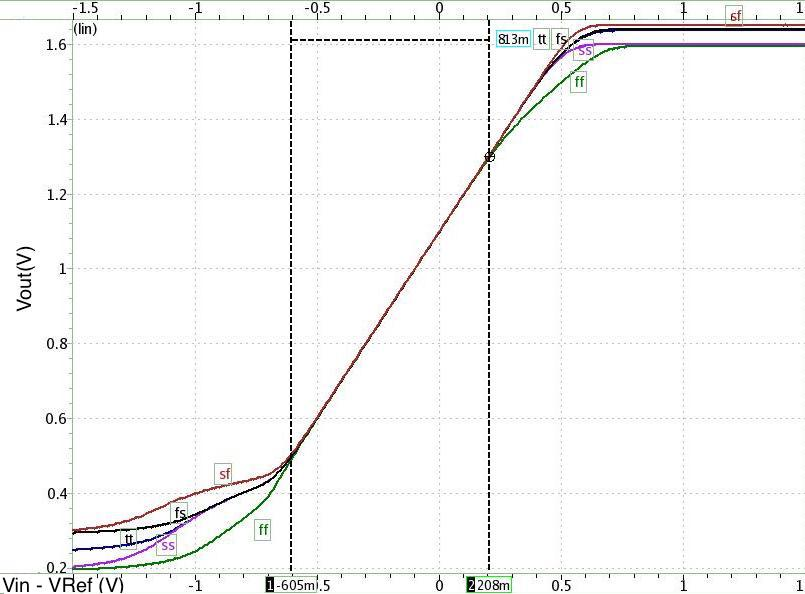
\includegraphics[width=0.9\textwidth] {images/chapter5/postSim/subtractor_5_xx.jpg}
        \raggedleft
        (a)
    \end{minipage}
    \vfill
    \begin{minipage}[t]{1\textwidth}
        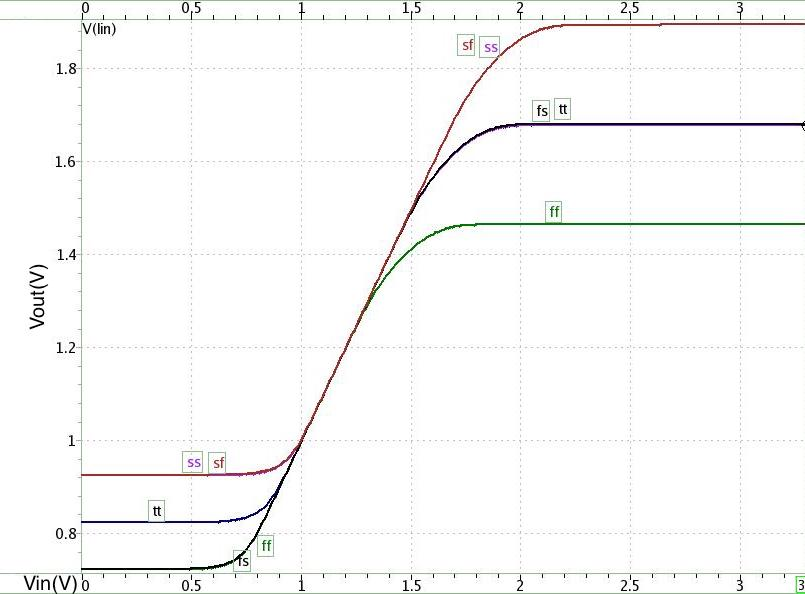
\includegraphics[width=0.9\textwidth] {images/chapter5/postSim/subtractor_5_zz.jpg}
        \raggedleft
        (b)
    \end{minipage}
    \caption{DC response of the output of our analog subtractor. (a)The x-axis is the difference between positive input and negative input ($V_x - V_{Ref}$). (b) The x-axis is the voltage of $V_z$ }
    \label{fig:sim:subtractor}
\end{figure}


\begin{table}[!htb]
    {\fontfamily{}\fontsize{10}{14}\selectfont
    \centering
    \begin{tabular}{l|c|c}
        VDD & \multicolumn{2}{|c}{$3.3V$}\\
        Ibias & \multicolumn{2}{|c}{$40\mu A$}\\
        Output voltage dynamic range & \multicolumn{2}{|c}{$0.2V$-$2.5V$}\\
        \hline
        \hline
        Input voltage type & $V_x$ & $V_z$\\
        \cline{2-3}
        Input Dynamic Range & from $V_{Ref} - 0.57V$ to $V_{Ref} + 0.2V$ & from $1V$ to $1.38V$ \\
        Bandwidth & $675k Hz$& irrelevant \\
        SNR (@10Hz) & $8.3e10$ & $8.4e10$ \\
    \end{tabular}
    \caption{The summary table of the analog subtracter circuit.}
    \label{tb:Subtractor}
    }
\end{table}

\subsection{Non-inverting Resistor-based Amplifier}

In Fig.\ref{fig:subtractor}, the Op2 along with the resistors (Ro, Ri1, Ri2) and the switches (Switch1, Switch2) compose our non-inverting resistor-based Amplifier.
We adopt this simple structure to amplify the output signal of the subtractor.
When the subtractor sends a small signal $\Delta v$ into Vin, the output voltage ($v_{out}$) is:
\begin{align}
    v_{out} &= (\Delta v - v_f) \times A_{Op2} \\
    v_f &= v_{out} \frac{R_i}{R_o + R_i} \\
    \frac{v_{out}}{\Delta v} &= \frac{A_{Op2}}{1 + A_{Op2}\frac{R_i}{R_i + R_o}} \\
    &\approx \frac{R_i + R_o}{R_i} \quad \text{For} \quad \frac{R_iA_{Op2}}{R_i + R_o} > 10 \label{eq:ResAmp}
\end{align}
The $R_i$ can be  $110k\Omega$ or $9.2k\Omega$ ($10k\Omega||110k\Omega$).
When two switches is off, the circuit acts like an unit-gain buffer.
Eq.(\ref{eq:ResAmp}) suggests that $A_{Op2}$ should be larger than 1000 (60dB).
Thus, the Op2 in Fig.\ref{fig:secondStage} adopts the structure of a two-stage amplifier (same with the operational amplifier in TIA block) due to its high gain and wide output dynamic range.


\begin{figure}[tb]
    \begin{minipage}[t]{0.47\textwidth}
        \centering
        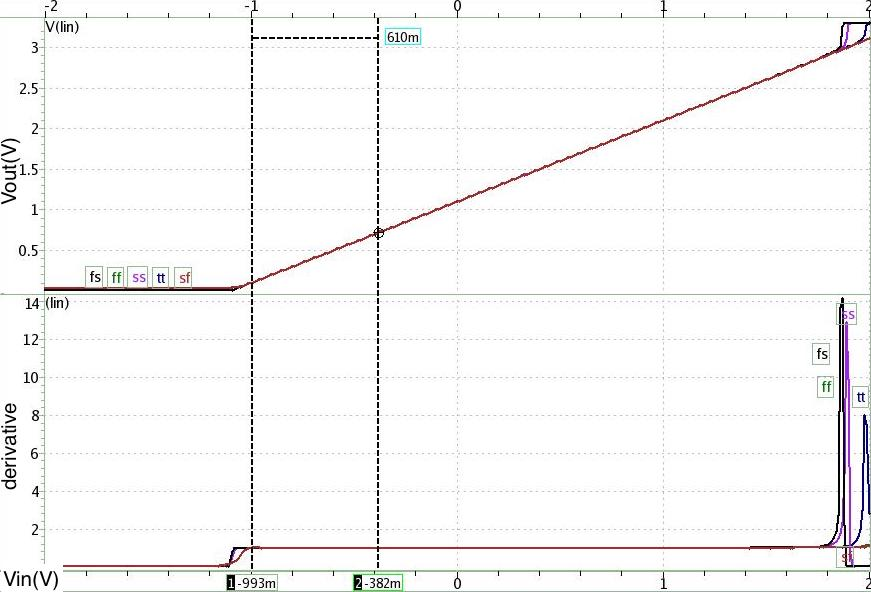
\includegraphics[width=1\textwidth] {images/chapter5/postSim/ResAmp_1x.PNG}
        (a)
    \end{minipage}
    % \hspace{8cm}
    \begin{minipage}[t]{0.47\textwidth}
        \centering
        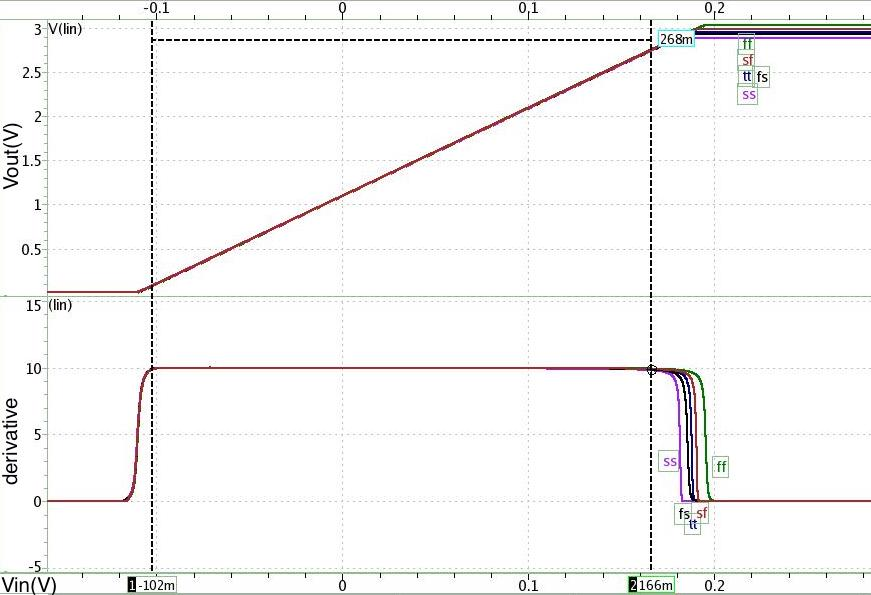
\includegraphics[width=1\textwidth] {images/chapter5/postSim/ResAmp_10x.PNG}
        (b)
    \end{minipage}
    \begin{minipage}[t]{1\textwidth}
        \centering
        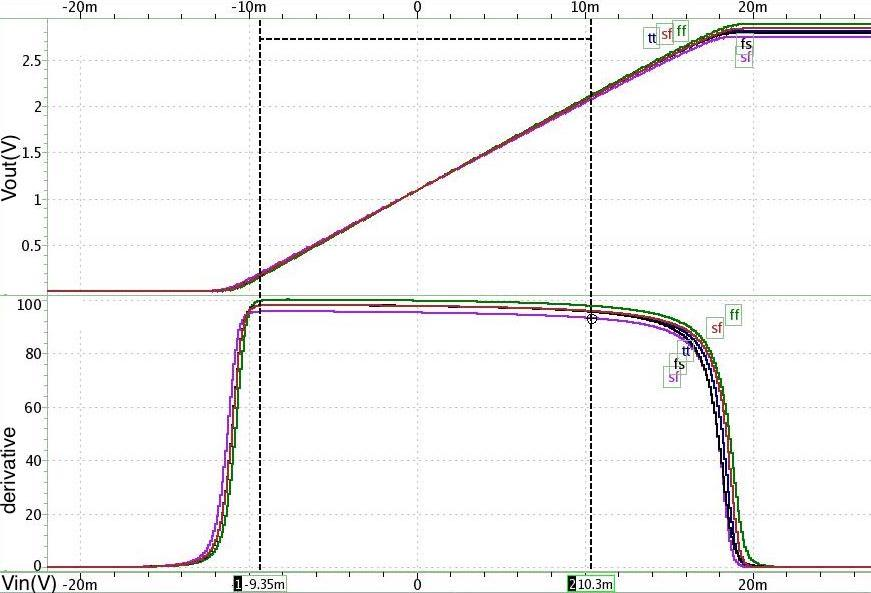
\includegraphics[width=0.47\textwidth] {images/chapter5/postSim/ResAmp_100x.PNG}
        (c)
    \end{minipage}
    \caption{Five corners output DC response (vout) and derivative ($dvout/dvin$) when being operated under the amplification rate of (a)1, (b)10, (c)100.}
    \label{fig:sim:ResAmp}
\end{figure}


\begin{table}[!hb]
    {\fontfamily{}\fontsize{10}{14}\selectfont
    \centering
    \begin{tabular}{l|c|c|c}
        Amplification Rate & 100 & 10 & 1\\
        \hline
        Error & < 7\% & < 0.7\% & < 0.02\% \\
        \hline
        Bandwidth & $10.1k$ Hz & $24k$ Hz & $220k$ Hz\\
        \hline
        Phase Margin & $110$ degree & $110$ degree & $84$ degree \\
        \hline
        Input Dynamic Range & from $-9mV$ to $17mV$ & from $-0.11V$ to $0.14V$ & from $-1.06$ to $1.9V$\\
        \hline
        Output Dynamic Range & \multicolumn{3}{c}{$0.1V$ - $3V$}\\
    \end{tabular}
    \caption{The summary table of simulation results.}
    \label{tb:sim:ResAmp}
    }
\end{table}


\emphy{One thing to note is that the derivation above views the $V_z$ as the virtual ground.
$V_z$ is both the input and output offset voltage of the amplifier.
It is usually applied with $1.1V$.
As mentioned in the subtractor section (Section.\ref{sec:sub}), the subtractor increases the output dynamic range of the amplifier stage.
If the subtractor is removed, the output offset voltage of this stage would be $V_{Ref}$, which is much lower ($\sim 0.8V$), and is changeable due to the process variation.}

Fig.\ref{fig:sim:ResAmp} presents the five corners post-simulation results of the amplifier and Table.\ref{tb:sim:ResAmp} is the summary table.
We swept the input and measured the output under three amplification gain.






% \FloatBarrier

\section{Post-simulation Result of Transient Measurement mode}
As mentioned in section.\ref{sec:TrM}, there are two usage of Transient Measurement mode (Fig.\ref{fig:ACmode}).
There simulation results are presented separately below.

\subsection{Detecting signals of biomolecules at the gate}

\begin{figure}[!htbp]
    \centering
        \includegraphics[width=0.7\textwidth] {images/chapter5/NWROC_block_vg.png}
    \caption{The block diagram of the Transient Measurement circuit. We simulate it by sending ac signal through the voltage source Vg.}
    \label{fig:Nblockvg}
\end{figure}

The first usage is to detect the output response of input voltage signal at gate.
The voltage signal is caused by the the biomolecule concentration.
This measurement is usually preceded by DC-sweep mode, which initializes the $I_D$ with the value of Ibias and set $g_m$ to a corresponding value.
Therefore, we replaced the transistor by a current signal Iin as in Fig.\ref{fig:Nblockvg}.
The ac signal is applied from Iin to perform the ac analysis.

\begin{figure}[!htb]
    \centering
        \includegraphics[width=1\textwidth] {images/chapter5/postSim/totalGain.PNG}
    \caption{The gain of $\frac{V_{out}}{I_{in}}$ when the voltage gain of the second stage is 100.}
    \label{fig:sim:vgGain}
\end{figure}

\begin{figure}[!htb]
    \centering
        \includegraphics[width=0.7\textwidth] {images/chapter5/postSim/noise.png}
    \caption{The input referred noise when the amplification rate of the second stage is 100.}
    \label{fig:sim:vgnoise}
\end{figure}

\emphy{Fig.\ref{fig:sim:vgGain} presents the maximal gain that the circuit provides at five corners.
Fig.\ref{fig:sim:vgnoise} shows the input referred noise.
The design specification requires the gain to be greater than $5M$ and the voltage noise referred to the gate of nanowire to be smaller than $2mV$.
The summary table (Table.\ref{tb:sim:vg}) computed the noise result by considering the $g_m$ as $1\mu$, which is the minimum $g_m$ that may exist in our measurement.}


\begin{table}[!htb]
    {\fontfamily{}\fontsize{10}{14}\selectfont
    \centering
    \begin{tabular}{l|c|c}
        & Design Spec. (Table.\ref{tb:ACSpec}) & Simulation Result \\
        \hline
        \hline
        $I_D$ Range & \multicolumn{2}{c}{$600n A$ - $10\mu A$}  \\
        \hline
        $gm$ Range & \multicolumn{2}{c}{$1\mu$ - $20\mu$}  \\
        \hline
        $\Delta V_G $ & \multicolumn{2}{c}{$20m V$ - $280m V$}  \\
        \hline
        Dynamic Input Current Range & $\pm 2.8\mu A$ & $6\mu A$-$-10\mu A$ \\
        \hline
        Maximal Amplification Rate ($\frac{V}{A}$)& $5M$ & $10.3M$\\
        \hline
        Bandwidth & $> 1k$Hz & $10.1k$Hz \\
        \hline
        Input Referred Noise ($V_G$) & $< 2m V$ & $ = \frac{0.291n}{1\mu}$ = $0.29m V$ @1Hz
    \end{tabular}
    \caption{The summary table. The first three rows are the nanowire chracteristics when applied with Transient Measurement mode.
    Others are the simulation results comparing with the design specification.}
    \label{tb:sim:vg}
    }
\end{table}

To be noted that in the simulation of Fig.\ref{fig:sim:vgnoise}, Ibias provides $10\mu A$ which is the largest biasing current in transient measurement mode (Table.\ref{tb:ACinput}).
This should be when the circuit has largest noise.

\subsection{Modulating biomolecule signals from the source terminal}
\begin{figure}[!htbp]
    \centering
        \includegraphics[width=0.7\textwidth] {images/chapter5/NWROC_block_vs.png}
    \caption{The block diagram of Transient Measurement circuit. We simulate it by sending ac signal to the source of the nanowire.}
    \label{fig:Nblockvs}
\end{figure}

The second usage of Transient Measurement mode is to apply a sinusoidal signal at the source of nanowire.
Vg and Ibias are kept constant during the measurement.
The output voltage is measured and used for computing the $g_m$ of the element.
\begin{equation}
    g_m = \frac{V_{out}}{v_s \times R_{TIA} \times A_{second}}
\end{equation}
$v_s$ is the amplitude of the input sinusoidal signal.
$A_{second}$ is the voltage gain of the second stage circuit and $R_{TIA}$ is the transimpedance of TIA in the froted circuit.

One thing to be noted is the offset voltage of the output.
The biomolecule concentration difference changes the $I_D$ of nanowire.
This $I_D$ difference not only results in the change of $g_m$ but also alters the offset current flowing through $R_{TIA}$.
This current is also amplified and may cause too much current flowing into the circuit.
The solution is to utilize Ibias to cancel the offset current.

Two simulation results presented below are the transient responses of the output voltage when $A_{amp}$ is 10 (Fig.\ref{fig:sim:sine10})and 100(Fig.\ref{fig:sim:sine100}).
$g_m$ of the transistor is swept in the same time.
According to the specification given in chapter 3 (Table.\ref{tb:ACSpec}), $g_m$ ranges from $1\mu$ to $10\mu$ in transient measurement.
The input sinusoidal signal has a frequency of $1k$Hz and an amplitude of $20mV$.
Their corresponding ac sweeps are presented in Fig.\ref{fig:sim:sine10_ac} and Fig.\ref{fig:sim:sine100_ac}.
\emphy{These results show that the circuit bandwidth is about $10k Hz$, which is caused by the last amplifier block.}
% 在紙本上註明一下之前說pole在source部分這件事是錯的


\begin{figure}[!htbp]
    \centering
        \includegraphics[width=1\textwidth] {images/chapter5/postSim/sine_gm_x10_1u_10u_tran.PNG}
    \caption{The transient analysis. The gain of $A_{amp}$ is 10. The $g_m$ is swept from $1\mu$ to $10\mu$.}
    \label{fig:sim:sine10}
\end{figure}
\begin{figure}[!htbp]
    \centering
        \includegraphics[width=1\textwidth] {images/chapter5/postSim/sine_gm_x10_1u_10u_ac.PNG}
    \caption{The ac analysis of the transient simulation result in Fig.\ref{fig:sim:sine10}.}
    \label{fig:sim:sine10_ac}
\end{figure}

\begin{figure}[!htbp]
    \centering
        \includegraphics[width=1\textwidth] {images/chapter5/postSim/sine_gm_x100_1u_6u_tran.PNG}
    \caption{The transient analysis. The gain of $A_{amp}$ is 100. The $g_m$ is swept from $1\mu$ to $6\mu$. There are two curves have the output saturation problem. This is because of the offset current flowing through $R_{TIA}$. It can be solved by increasing the current provided by Ibias.}
    \label{fig:sim:sine100}
\end{figure}
\begin{figure}[!htbp]
    \centering
        \includegraphics[width=1\textwidth] {images/chapter5/postSim/sine_gm_x100_1u_6u_ac.PNG}
    \caption{The ac analysis of the transient simulation result in Fig.\ref{fig:sim:sine100}.}
    \label{fig:sim:sine100_ac}
\end{figure}





%